\section{Results:}
\subsection{Results using BDRS + Filtering.}

We use the following color convention for graphs through out the document:
\begin{center}
    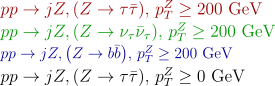
\includegraphics[width=0.5\textwidth]{./ColorConventions.pdf}
\end{center}
We present some simple results obtained using jet substructure variables on jets tagged using BDRS+Filtering methods (Note: we use the final 2 step filtered (BDRS\cite{BDRS}+filtering) jet to evaluate variables and all of these results are for events with MPI enabled). Note that planar flow \cite{PlanarFlow} [\autoref{fig:PlanarFlow}, \autoref{fig:PlanarFlowX}] seem to work extremely well.

\begin{figure}[H]
    \begin{center}
        \includegraphics[width=0.7\textwidth]{./EFrac.pdf}
        \caption{ Electromagnetic energy fraction of the jet, normalized to unit area under the curve. }
        \label{fig:EFrac}
    \end{center}
\end{figure}

\begin{figure}[H]
    \begin{center}
        \includegraphics[width=0.7\textwidth]{./HFrac.pdf}
        \caption{ Hadronic energy fraction of the jet, normalized to unit area under the curve. }
        \label{fig:HFrac}
    \end{center}
\end{figure}

\begin{figure}[H]
    \begin{center}
        \includegraphics[width=0.7\textwidth]{./NTracks.pdf}
        \caption{ Number of tracks in the jet, normalized to unit area under the curve. }
        \label{fig:NTracks}
    \end{center}
\end{figure}

\begin{figure}[H]
    \begin{center}
        \includegraphics[width=0.7\textwidth]{./Masses.pdf}
        \caption{ Masses of the jet after BDRS and filtering steps, normalized to unit area under the curve. }
        \label{fig:Masses}
    \end{center}
\end{figure}

\begin{figure}[H]
    \begin{center}
        \includegraphics[width=0.7\textwidth]{./PlanarFlow.pdf}
        \caption{ Planar Flow of the jet after BDRS and filtering steps, normalized to unit area under the curve. }
        \label{fig:PlanarFlow}
    \end{center}
\end{figure}

\begin{figure}[H]
    \begin{center}
        \includegraphics[width=0.49\textwidth]{./PlanarFlow1.pdf}
        \includegraphics[width=0.49\textwidth]{./PlanarFlow2.pdf}\\
        \caption{ Planar Flow of the two subjets after BDRS and filtering steps, normalized to unit area under the curve. }
        \label{fig:PlanarFlowX}
    \end{center}
\end{figure}

\begin{figure}[H]
    \begin{center}
        \includegraphics[width=0.49\textwidth]{./NSub1.pdf}
        \includegraphics[width=0.49\textwidth]{./NSub2.pdf}\\
        \includegraphics[width=0.49\textwidth]{./NSub3.pdf}
        \includegraphics[width=0.49\textwidth]{./NSub4.pdf}\\
        \caption{ {\tt NSubJettiness} observable, normalized to unit area under the curve. }
        \label{fig:NSub}
    \end{center}
\end{figure}

\begin{figure}[H]
    \begin{center}
        \includegraphics[width=0.49\textwidth]{./NSubRatio1.pdf}
        \includegraphics[width=0.49\textwidth]{./NSubRatio2.pdf}\\
        \includegraphics[width=0.49\textwidth]{./NSubRatio3.pdf}
        \includegraphics[width=0.49\textwidth]{./NSubRatio4.pdf}\\
        \caption{ Ratio of {\tt NSubJettiness} observable, normalized to unit area under the curve. }
        \label{fig:NSubRatio}
    \end{center}
\end{figure}

\begin{figure}[H]
    \begin{center}
        \includegraphics[width=0.49\textwidth]{./ECorr1.pdf}
        \includegraphics[width=0.49\textwidth]{./ECorr2.pdf}\\
        \includegraphics[width=0.49\textwidth]{./ECorr3.pdf}
        \includegraphics[width=0.49\textwidth]{./ECorr4.pdf}\\
        \includegraphics[width=0.49\textwidth]{./ECorr5.pdf}
        \includegraphics[width=0.49\textwidth]{./ECorr6.pdf}\\
        \caption{ Energy Correlation observable, normalized to unit area under the curve. }
        \label{fig:ECorr}
    \end{center}
\end{figure}

\begin{figure}[H]
    \begin{center}
        \includegraphics[width=0.49\textwidth]{./ECorrDR1.pdf}
        \includegraphics[width=0.49\textwidth]{./ECorrDR2.pdf}\\
        \includegraphics[width=0.49\textwidth]{./ECorrDR3.pdf}
        \includegraphics[width=0.49\textwidth]{./ECorrDR4.pdf}\\
        \caption{ Energy Correlation double ratio observable, normalized to unit area under the curve. }
        \label{fig:ECorrDR}
    \end{center}
\end{figure}

\begin{figure}[H]
    \begin{center}
        \includegraphics[width=0.49\textwidth]{./T1NSub1vsPf.pdf}
        \includegraphics[width=0.49\textwidth]{./T1NSub2vsPf.pdf}\\
        \includegraphics[width=0.49\textwidth]{./T1NSub3vsPf.pdf}
        \includegraphics[width=0.49\textwidth]{./T1NSub4vsPf.pdf}\\
        \caption{ {\tt NSubjettiness} (x-axis) vs planar flow (y-axis) for boosted $jZ\rightarrow \tau \bar{\tau}$ }
        \label{fig:nsubvspf1}
    \end{center}
\end{figure}

\begin{figure}[H]
    \begin{center}
        \includegraphics[width=0.49\textwidth]{./T2NSub1vsPf.pdf}
        \includegraphics[width=0.49\textwidth]{./T2NSub2vsPf.pdf}\\
        \includegraphics[width=0.49\textwidth]{./T2NSub3vsPf.pdf}
        \includegraphics[width=0.49\textwidth]{./T2NSub4vsPf.pdf}\\
        \caption{ {\tt NSubjettiness} (x-axis) vs planar flow (y-axis) for boosted $jZ\rightarrow \nu \bar{\nu}$ }
        \label{fig:nsubvspf2}
    \end{center}
\end{figure}

\begin{figure}[H]
    \begin{center}
        \includegraphics[width=0.49\textwidth]{./T3NSub1vsPf.pdf}
        \includegraphics[width=0.49\textwidth]{./T3NSub2vsPf.pdf}\\
        \includegraphics[width=0.49\textwidth]{./T3NSub3vsPf.pdf}
        \includegraphics[width=0.49\textwidth]{./T3NSub4vsPf.pdf}\\
        \caption{ {\tt NSubjettiness} (x-axis) vs planar flow (y-axis) for boosted $jZ\rightarrow b \bar{b}$ }
        \label{fig:nsubvspf3}
    \end{center}
\end{figure}

\begin{figure}[H]
    \begin{center}
        \includegraphics[width=0.49\textwidth]{./T4NSub1vsPf.pdf}
        \includegraphics[width=0.49\textwidth]{./T4NSub2vsPf.pdf}\\
        \includegraphics[width=0.49\textwidth]{./T4NSub3vsPf.pdf}
        \includegraphics[width=0.49\textwidth]{./T4NSub4vsPf.pdf}\\
        \caption{ {\tt NSubjettiness} (x-axis) vs planar flow (y-axis) for unboosted $jZ\rightarrow \tau \bar{\tau}$ }
        \label{fig:nsubvspf4}
    \end{center}
\end{figure}

{\newpage}

\subsubsection{Analyzing planar flow:}

We suspect Planar Flow might be correlated with {\tt NSubjettiness}, to verify these, we check the following graphs [\autoref{fig:nsubvspf1}, \autoref{fig:nsubvspf2}, \autoref{fig:nsubvspf3}, \autoref{fig:nsubvspf4}], as can be seen there seems to be some correlation, we quantify this:

\begin{eqnarray*}
    J & \equiv & \text{The }Z-\text{tagged jet obtained after BDRS + Filtering.}\\
    J_{1} & \equiv & \text{The highest }p_{T}\text{ subjet of }J.\\
    J_{2} & \equiv & \text{The other subjet of }J.\\
    P_{f} & \equiv & \text{Planar Flow}.\\
    \tau_{N} & \equiv & n^{th}\text{ NSubjettiness}.\\
    S\left(J\right) & \equiv & \sum_{i\in J}p_{T_{i}}\Delta R\left(i,J\right)\\
    \\
    \left\langle P_{f}\left(J\right),\tau_{2}\left(J\right)\right\rangle  & = & 3.70\times10^{-2}\\
    \left\langle P_{f}\left(J\right),\tau_{3}\left(J\right)\right\rangle  & = & 4.26\times10^{-2}\\
    \left\langle P_{f}\left(J\right),\tau_{4}\left(J\right)\right\rangle  & = & 4.32\times10^{-2}\\
    \left\langle P_{f}\left(J\right),\tau_{5}\left(J\right)\right\rangle  & = & 4.20\times10^{-2}\\
    \left\langle P_{f}\left(J\right),S\left(J\right)\right\rangle  & = & 9.73\times10^{-3}\\
    \\
    \left\langle P_{f}\left(J_{1}\right),\tau_{2}\left(J_{1}\right)\right\rangle  & = & 2.37\times10^{-1}\\
    \left\langle P_{f}\left(J_{1}\right),\tau_{3}\left(J_{1}\right)\right\rangle  & = & 2.37\times10^{-1}\\
    \left\langle P_{f}\left(J_{1}\right),\tau_{4}\left(J_{1}\right)\right\rangle  & = & 2.26\times10^{-1}\\
    \left\langle P_{f}\left(J_{1}\right),\tau_{5}\left(J_{1}\right)\right\rangle  & = & 2.15\times10^{-1}\\
    \left\langle P_{f}\left(J_{1}\right),S\left(J_{1}\right)\right\rangle  & = & 2.88\times10^{-1}\\
    \\
    \left\langle P_{f}\left(J_{2}\right),\tau_{2}\left(J_{2}\right)\right\rangle  & = & 2.32\times10^{-1}\\
    \left\langle P_{f}\left(J_{2}\right),\tau_{3}\left(J_{2}\right)\right\rangle  & = & 2.19\times10^{-1}\\
    \left\langle P_{f}\left(J_{2}\right),\tau_{4}\left(J_{2}\right)\right\rangle  & = & 2.00\times10^{-1}\\
    \left\langle P_{f}\left(J_{2}\right),\tau_{5}\left(J_{2}\right)\right\rangle  & = & 1.83\times10^{-1}\\
    \left\langle P_{f}\left(J_{2}\right),S\left(J_{2}\right)\right\rangle  & = & 2.72\times10^{-1}\\
\end{eqnarray*}

\begin{figure}[H]
    \begin{center}
        \includegraphics[width=0.7\textwidth]{./Spread0.pdf}
        \caption{ The variable $S\left(J\right)$  }
        \label{fig:Spread0}
    \end{center}
\end{figure}

\begin{figure}[H]
    \begin{center}
        \includegraphics[width=0.49\textwidth]{./Spread1.pdf}
        \includegraphics[width=0.49\textwidth]{./Spread2.pdf}\\
        \caption{ The variable $S\left(J_1\right)$  and $S\left(J_2\right)$ }
        \label{fig:SpreadX}
    \end{center}
\end{figure}

The definition of planar flow (from \cite{PlanarFlow}) is:

\begin{eqnarray*}
	I_{w}^{kl} & \equiv & \frac{1}{m_{J}}\sum_{i}w_{i}\frac{p_{ik}}{w_{i}}\frac{p_{il}}{w_{i}}\\
	P_{f} & = & \frac{4\det\left(I_{w}\right)}{\text{tr}\left(I_{w}\right)^{2}}
\end{eqnarray*}

we can recast this in the following form:

% Preview body

\begin{eqnarray*}
	\vec{A} & \equiv & \left(\begin{array}{c}
		p_{1,1}/\sqrt{w_{1}}\\
		p_{2,1}/\sqrt{w_{2}}\\
		\vdots\\
		p_{N,1}/\sqrt{w_{N}}
	\end{array}\right)\\
	\vec{B} & \equiv & \left(\begin{array}{c}
		p_{1,2}/\sqrt{w_{1}}\\
		p_{2,2}/\sqrt{w_{2}}\\
		\vdots\\
		p_{N,2}/\sqrt{w_{N}}
	\end{array}\right)\\
	\text{So:}\\
	A_{i} & = & p_{i,1}/\sqrt{w_{i}}\\
	B_{i} & = & p_{i,2}/\sqrt{w_{i}}
\end{eqnarray*}

Now the matrix $I_{w}$ becomes:

\begin{eqnarray*}
	I_{w} & = & \frac{1}{m_{J}}\left(\begin{array}{cc}
		\vec{A}\cdot\vec{A} & \vec{A}\cdot\vec{B}\\
		\vec{A}\cdot\vec{B} & \vec{B}\cdot\vec{B}
	\end{array}\right)\equiv\left(\begin{array}{cc}
		\left|\left|\vec{A}\right|\right|^{2} & \vec{A}\cdot\vec{B}\\
		\vec{A}\cdot\vec{B} & \left|\left|\vec{B}\right|\right|^{2}
	\end{array}\right)\\
	P_{f} & = & \frac{4\left[\left|\left|\vec{A}\right|\right|^{2}\left|\left|\vec{B}\right|\right|^{2}-\left(\vec{A}\cdot\vec{B}\right)^{2}\right]}{\left(\left|\left|\vec{A}\right|\right|^{2}+\left|\left|\vec{B}\right|\right|^{2}\right)^{2}}\\
	\text{Define:}\\
	\cos\left(\theta\right) & \equiv & \frac{\left(\vec{A}\cdot\vec{B}\right)}{\left|\left|\vec{A}\right|\right|\left|\left|\vec{B}\right|\right|}\\
	\text{Then:}\\
	P_{f} & = & \frac{4\left[\left|\left|\vec{A}\right|\right|^{2}\left|\left|\vec{B}\right|\right|^{2}-\left(\vec{A}\cdot\vec{B}\right)^{2}\right]}{\left(\left|\left|\vec{A}\right|\right|^{4}+\left|\left|\vec{B}\right|\right|^{4}+2\left|\left|\vec{A}\right|\right|^{2}\left|\left|\vec{B}\right|\right|^{2}\right)}\\
	& = & \frac{\left|\left|\vec{A}\right|\right|^{2}\left|\left|\vec{B}\right|\right|^{2}\left[4\left(1-\cos^{2}\left(\theta\right)\right)\right]}{\left|\left|\vec{A}\right|\right|^{2}\left|\left|\vec{B}\right|\right|^{2}\left(\frac{\left|\left|\vec{A}\right|\right|^{2}}{\left|\left|\vec{B}\right|\right|^{2}}+\frac{\left|\left|\vec{B}\right|\right|^{2}}{\left|\left|\vec{A}\right|\right|^{2}}+2\right)}\\
	P_{f} & = & \frac{4\left[1-\cos^{2}\left(\theta\right)\right]}{\frac{\left|\left|\vec{A}\right|\right|^{2}}{\left|\left|\vec{B}\right|\right|^{2}}+\frac{\left|\left|\vec{B}\right|\right|^{2}}{\left|\left|\vec{A}\right|\right|^{2}}+2}
\end{eqnarray*}

In this form, analyzing Planar Flow becomes much easier.

$P_{f}$ is small when denominator is large {[}either $\left|\left|\vec{A}\right|\right|\rightarrow0$ or $\left|\left|\vec{B}\right|\right|\rightarrow0$ or both{]} or when numerator is small {[}$\cos^{2}\left(\theta\right)\rightarrow1${]}, we will be more interested in the former case (the later is useful in explaining why QCD has smaller $P_{f}$ compared to say $t\bar{t}$).

If all the constituent particles (in the jet) from a decay lie along a line (in a plane transverse to the momentum vector of the jet), then we can choose the basis (by Gram Schmidt) such that either $\vec{A}=0$ or $\vec{B}=0$ and hence the denominator $\rightarrow\infty$.

\subsubsection{Kinematics of jets from $\tau$ decay:}

\begin{figure}[H]
	\begin{center}
		\includegraphics[width=0.7\textwidth]{TauJet.pdf}
		\caption{Schematic of a hadronically decaying $\tau$.}
		\label{fig:TauDecay}
	\end{center}
\end{figure}

\begin{figure}[H]
	\begin{center}
		\includegraphics[height=0.2\textheight]{Transverse.pdf}
		\caption{Momentum distribution of the $\tau$ decay products in the transverse (to the jet momentum) plane.}
		\label{fig:VectorDist}
	\end{center}
\end{figure}

All the (visible) constituents from a (hadronic) $\tau$ decay come from the virtual $W^{\pm}$ and are color connected [\autoref{fig:TauDecay}] $\Rightarrow$ they all lie on a line in the plane transverse to the jet [\autoref{fig:VectorDist}], hence either $\left| \left| \vec{A}  \right|  \right|$ or $\left| \left| \vec{B}  \right|  \right|$ $\rightarrow$ 0 and hence $P_f \rightarrow 0$.